\section{moeo\-Easy\-EA$<$ MOEOT $>$ Class Template Reference}
\label{classmoeoEasyEA}\index{moeoEasyEA@{moeoEasyEA}}
An easy class to design multi-objective evolutionary algorithms.  


{\tt \#include $<$moeo\-Easy\-EA.h$>$}

Inheritance diagram for moeo\-Easy\-EA$<$ MOEOT $>$::\begin{figure}[H]
\begin{center}
\leavevmode
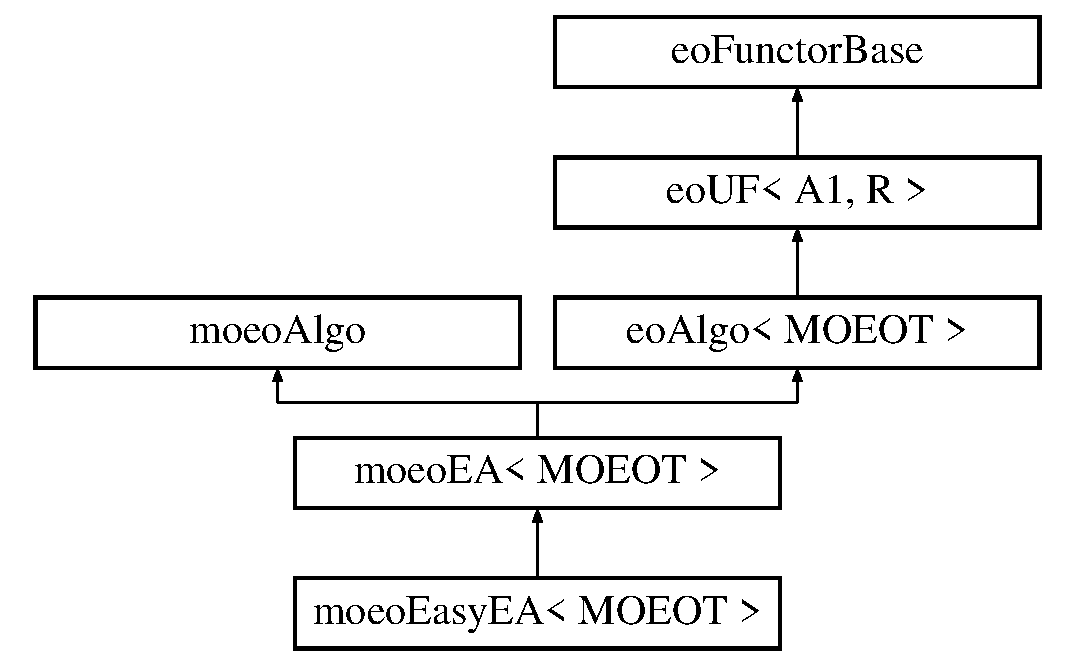
\includegraphics[height=5cm]{classmoeoEasyEA}
\end{center}
\end{figure}
\subsection*{Public Member Functions}
\begin{CompactItemize}
\item 
\bf{moeo\-Easy\-EA} (\bf{eo\-Continue}$<$ MOEOT $>$ \&\_\-continuator, \bf{eo\-Eval\-Func}$<$ MOEOT $>$ \&\_\-eval, \bf{eo\-Breed}$<$ MOEOT $>$ \&\_\-breed, \bf{moeo\-Replacement}$<$ MOEOT $>$ \&\_\-replace, \bf{moeo\-Fitness\-Assignment}$<$ MOEOT $>$ \&\_\-fitness\-Eval, \bf{moeo\-Diversity\-Assignment}$<$ MOEOT $>$ \&\_\-diversity\-Eval, bool \_\-eval\-Fit\-And\-Div\-Before\-Selection=false)
\begin{CompactList}\small\item\em Ctor taking a breed and merge. \item\end{CompactList}\item 
\bf{moeo\-Easy\-EA} (\bf{eo\-Continue}$<$ MOEOT $>$ \&\_\-continuator, \bf{eo\-Pop\-Eval\-Func}$<$ MOEOT $>$ \&\_\-pop\-Eval, \bf{eo\-Breed}$<$ MOEOT $>$ \&\_\-breed, \bf{moeo\-Replacement}$<$ MOEOT $>$ \&\_\-replace, \bf{moeo\-Fitness\-Assignment}$<$ MOEOT $>$ \&\_\-fitness\-Eval, \bf{moeo\-Diversity\-Assignment}$<$ MOEOT $>$ \&\_\-diversity\-Eval, bool \_\-eval\-Fit\-And\-Div\-Before\-Selection=false)
\begin{CompactList}\small\item\em Ctor taking a breed, a merge and a eo\-Pop\-Eval. \item\end{CompactList}\item 
\bf{moeo\-Easy\-EA} (\bf{eo\-Continue}$<$ MOEOT $>$ \&\_\-continuator, \bf{eo\-Eval\-Func}$<$ MOEOT $>$ \&\_\-eval, \bf{eo\-Breed}$<$ MOEOT $>$ \&\_\-breed, \bf{eo\-Merge}$<$ MOEOT $>$ \&\_\-merge, \bf{eo\-Reduce}$<$ MOEOT $>$ \&\_\-reduce, \bf{moeo\-Fitness\-Assignment}$<$ MOEOT $>$ \&\_\-fitness\-Eval, \bf{moeo\-Diversity\-Assignment}$<$ MOEOT $>$ \&\_\-diversity\-Eval, bool \_\-eval\-Fit\-And\-Div\-Before\-Selection=false)
\begin{CompactList}\small\item\em Ctor taking a breed, a merge and a reduce. \item\end{CompactList}\item 
\bf{moeo\-Easy\-EA} (\bf{eo\-Continue}$<$ MOEOT $>$ \&\_\-continuator, \bf{eo\-Eval\-Func}$<$ MOEOT $>$ \&\_\-eval, \bf{eo\-Select}$<$ MOEOT $>$ \&\_\-select, \bf{eo\-Transform}$<$ MOEOT $>$ \&\_\-transform, \bf{moeo\-Replacement}$<$ MOEOT $>$ \&\_\-replace, \bf{moeo\-Fitness\-Assignment}$<$ MOEOT $>$ \&\_\-fitness\-Eval, \bf{moeo\-Diversity\-Assignment}$<$ MOEOT $>$ \&\_\-diversity\-Eval, bool \_\-eval\-Fit\-And\-Div\-Before\-Selection=false)
\begin{CompactList}\small\item\em Ctor taking a select, a transform and a replacement. \item\end{CompactList}\item 
\bf{moeo\-Easy\-EA} (\bf{eo\-Continue}$<$ MOEOT $>$ \&\_\-continuator, \bf{eo\-Eval\-Func}$<$ MOEOT $>$ \&\_\-eval, \bf{eo\-Select}$<$ MOEOT $>$ \&\_\-select, \bf{eo\-Transform}$<$ MOEOT $>$ \&\_\-transform, \bf{eo\-Merge}$<$ MOEOT $>$ \&\_\-merge, \bf{eo\-Reduce}$<$ MOEOT $>$ \&\_\-reduce, \bf{moeo\-Fitness\-Assignment}$<$ MOEOT $>$ \&\_\-fitness\-Eval, \bf{moeo\-Diversity\-Assignment}$<$ MOEOT $>$ \&\_\-diversity\-Eval, bool \_\-eval\-Fit\-And\-Div\-Before\-Selection=false)
\begin{CompactList}\small\item\em Ctor taking a select, a transform, a merge and a reduce. \item\end{CompactList}\item 
virtual void \bf{operator()} (\bf{eo\-Pop}$<$ MOEOT $>$ \&\_\-pop)
\begin{CompactList}\small\item\em Applies a few generation of evolution to the population \_\-pop. \item\end{CompactList}\end{CompactItemize}
\subsection*{Protected Attributes}
\begin{CompactItemize}
\item 
\bf{eo\-Continue}$<$ MOEOT $>$ \& \bf{continuator}\label{classmoeoEasyEA_5f5b76acbaf99a6a3ee2710da07dde29}

\begin{CompactList}\small\item\em the stopping criteria \item\end{CompactList}\item 
\bf{eo\-Eval\-Func}$<$ MOEOT $>$ \& \bf{eval}\label{classmoeoEasyEA_26e8ebce6a1bc3216e20171688ba6b83}

\begin{CompactList}\small\item\em the evaluation functions \item\end{CompactList}\item 
\bf{eo\-Pop\-Loop\-Eval}$<$ MOEOT $>$ \bf{loop\-Eval}\label{classmoeoEasyEA_c1d492090805bf322c07159a9238a7ae}

\begin{CompactList}\small\item\em to evaluate the whole population \item\end{CompactList}\item 
\bf{eo\-Pop\-Eval\-Func}$<$ MOEOT $>$ \& \bf{pop\-Eval}\label{classmoeoEasyEA_189a8f5196844907ff71f386d95bf415}

\begin{CompactList}\small\item\em to evaluate the whole population \item\end{CompactList}\item 
\bf{eo\-Select\-Transform}$<$ MOEOT $>$ \bf{select\-Transform}\label{classmoeoEasyEA_bd69a176f3cacc2694342075a9022f74}

\begin{CompactList}\small\item\em breed: a select followed by a transform \item\end{CompactList}\item 
\bf{eo\-Breed}$<$ MOEOT $>$ \& \bf{breed}\label{classmoeoEasyEA_35d5909694019d1b0d52347c72a9092e}

\begin{CompactList}\small\item\em the breeder \item\end{CompactList}\item 
\bf{eo\-Merge\-Reduce}$<$ MOEOT $>$ \bf{merge\-Reduce}\label{classmoeoEasyEA_15a69654c07b24f9795add0a22f1f856}

\begin{CompactList}\small\item\em replacement: a merge followed by a reduce \item\end{CompactList}\item 
\bf{moeo\-Replacement}$<$ MOEOT $>$ \& \bf{replace}\label{classmoeoEasyEA_91611cf2862c2db953554e367a576244}

\begin{CompactList}\small\item\em the replacment strategy \item\end{CompactList}\item 
\bf{moeo\-Fitness\-Assignment}$<$ MOEOT $>$ \& \bf{fitness\-Eval}\label{classmoeoEasyEA_1268fc2f0b62fe51bca17d4efb51954b}

\begin{CompactList}\small\item\em the fitness assignment strategy \item\end{CompactList}\item 
\bf{moeo\-Diversity\-Assignment}$<$ MOEOT $>$ \& \bf{diversity\-Eval}\label{classmoeoEasyEA_b9d1b3790072dbbbe0012a252bab95f4}

\begin{CompactList}\small\item\em the diversity assignment strategy \item\end{CompactList}\item 
bool \bf{eval\-Fit\-And\-Div\-Before\-Selection}\label{classmoeoEasyEA_856a19d9a7c180fe33ce7a5bb010edcc}

\begin{CompactList}\small\item\em if this parameter is set to 'true', the fitness and the diversity of the whole population will be re-evaluated before the selection process \item\end{CompactList}\item 
\bf{moeo\-Easy\-EA::eo\-Dummy\-Eval} \bf{dummy\-Eval}\label{classmoeoEasyEA_16cbb12cb7de77c6d7d3f7aee9434880}

\begin{CompactList}\small\item\em a dummy eval \item\end{CompactList}\item 
\bf{moeo\-Easy\-EA::eo\-Dummy\-Select} \bf{dummy\-Select}\label{classmoeoEasyEA_fed6522fe0fcea204850dbb89cc7116e}

\begin{CompactList}\small\item\em a dummy select \item\end{CompactList}\item 
\bf{moeo\-Easy\-EA::eo\-Dummy\-Transform} \bf{dummy\-Transform}\label{classmoeoEasyEA_56991f36963ed61e44e91759c891f13c}

\begin{CompactList}\small\item\em a dummy transform \item\end{CompactList}\item 
\bf{eo\-No\-Elitism}$<$ MOEOT $>$ \bf{dummy\-Merge}\label{classmoeoEasyEA_e26830e1301cfd626eed55b0fbf8dbcb}

\begin{CompactList}\small\item\em a dummy merge \item\end{CompactList}\item 
\bf{eo\-Truncate}$<$ MOEOT $>$ \bf{dummy\-Reduce}\label{classmoeoEasyEA_65963f9308ccc0acc3dfc32a128f6228}

\begin{CompactList}\small\item\em a dummy reduce \item\end{CompactList}\end{CompactItemize}
\subsection*{Classes}
\begin{CompactItemize}
\item 
class \bf{eo\-Dummy\-Eval}
\begin{CompactList}\small\item\em a dummy eval \item\end{CompactList}\item 
class \bf{eo\-Dummy\-Select}
\begin{CompactList}\small\item\em a dummy select \item\end{CompactList}\item 
class \bf{eo\-Dummy\-Transform}
\begin{CompactList}\small\item\em a dummy transform \item\end{CompactList}\end{CompactItemize}


\subsection{Detailed Description}
\subsubsection*{template$<$class MOEOT$>$ class moeo\-Easy\-EA$<$ MOEOT $>$}

An easy class to design multi-objective evolutionary algorithms. 



Definition at line 58 of file moeo\-Easy\-EA.h.

\subsection{Constructor \& Destructor Documentation}
\index{moeoEasyEA@{moeo\-Easy\-EA}!moeoEasyEA@{moeoEasyEA}}
\index{moeoEasyEA@{moeoEasyEA}!moeoEasyEA@{moeo\-Easy\-EA}}
\subsubsection{\setlength{\rightskip}{0pt plus 5cm}template$<$class MOEOT$>$ \bf{moeo\-Easy\-EA}$<$ MOEOT $>$::\bf{moeo\-Easy\-EA} (\bf{eo\-Continue}$<$ MOEOT $>$ \& {\em \_\-continuator}, \bf{eo\-Eval\-Func}$<$ MOEOT $>$ \& {\em \_\-eval}, \bf{eo\-Breed}$<$ MOEOT $>$ \& {\em \_\-breed}, \bf{moeo\-Replacement}$<$ MOEOT $>$ \& {\em \_\-replace}, \bf{moeo\-Fitness\-Assignment}$<$ MOEOT $>$ \& {\em \_\-fitness\-Eval}, \bf{moeo\-Diversity\-Assignment}$<$ MOEOT $>$ \& {\em \_\-diversity\-Eval}, bool {\em \_\-eval\-Fit\-And\-Div\-Before\-Selection} = {\tt false})\hspace{0.3cm}{\tt  [inline]}}\label{classmoeoEasyEA_3f657699b8ed340ae3f51194206daa20}


Ctor taking a breed and merge. 

\begin{Desc}
\item[Parameters:]
\begin{description}
\item[{\em \_\-continuator}]the stopping criteria \item[{\em \_\-eval}]the evaluation functions \item[{\em \_\-breed}]the breeder \item[{\em \_\-replace}]the replacement strategy \item[{\em \_\-fitness\-Eval}]the fitness evaluation scheme \item[{\em \_\-diversity\-Eval}]the diversity evaluation scheme \item[{\em \_\-eval\-Fit\-And\-Div\-Before\-Selection}]put this parameter to 'true' if you want to re-evalue the fitness and the diversity of the population before the selection process \end{description}
\end{Desc}


Definition at line 72 of file moeo\-Easy\-EA.h.\index{moeoEasyEA@{moeo\-Easy\-EA}!moeoEasyEA@{moeoEasyEA}}
\index{moeoEasyEA@{moeoEasyEA}!moeoEasyEA@{moeo\-Easy\-EA}}
\subsubsection{\setlength{\rightskip}{0pt plus 5cm}template$<$class MOEOT$>$ \bf{moeo\-Easy\-EA}$<$ MOEOT $>$::\bf{moeo\-Easy\-EA} (\bf{eo\-Continue}$<$ MOEOT $>$ \& {\em \_\-continuator}, \bf{eo\-Pop\-Eval\-Func}$<$ MOEOT $>$ \& {\em \_\-pop\-Eval}, \bf{eo\-Breed}$<$ MOEOT $>$ \& {\em \_\-breed}, \bf{moeo\-Replacement}$<$ MOEOT $>$ \& {\em \_\-replace}, \bf{moeo\-Fitness\-Assignment}$<$ MOEOT $>$ \& {\em \_\-fitness\-Eval}, \bf{moeo\-Diversity\-Assignment}$<$ MOEOT $>$ \& {\em \_\-diversity\-Eval}, bool {\em \_\-eval\-Fit\-And\-Div\-Before\-Selection} = {\tt false})\hspace{0.3cm}{\tt  [inline]}}\label{classmoeoEasyEA_6cdebc72ce0134ce1680dafdf94740a1}


Ctor taking a breed, a merge and a eo\-Pop\-Eval. 

\begin{Desc}
\item[Parameters:]
\begin{description}
\item[{\em \_\-continuator}]the stopping criteria \item[{\em \_\-pop\-Eval}]the evaluation functions for the whole population \item[{\em \_\-breed}]the breeder \item[{\em \_\-replace}]the replacement strategy \item[{\em \_\-fitness\-Eval}]the fitness evaluation scheme \item[{\em \_\-diversity\-Eval}]the diversity evaluation scheme \item[{\em \_\-eval\-Fit\-And\-Div\-Before\-Selection}]put this parameter to 'true' if you want to re-evalue the fitness and the diversity of the population before the selection process \end{description}
\end{Desc}


Definition at line 90 of file moeo\-Easy\-EA.h.\index{moeoEasyEA@{moeo\-Easy\-EA}!moeoEasyEA@{moeoEasyEA}}
\index{moeoEasyEA@{moeoEasyEA}!moeoEasyEA@{moeo\-Easy\-EA}}
\subsubsection{\setlength{\rightskip}{0pt plus 5cm}template$<$class MOEOT$>$ \bf{moeo\-Easy\-EA}$<$ MOEOT $>$::\bf{moeo\-Easy\-EA} (\bf{eo\-Continue}$<$ MOEOT $>$ \& {\em \_\-continuator}, \bf{eo\-Eval\-Func}$<$ MOEOT $>$ \& {\em \_\-eval}, \bf{eo\-Breed}$<$ MOEOT $>$ \& {\em \_\-breed}, \bf{eo\-Merge}$<$ MOEOT $>$ \& {\em \_\-merge}, \bf{eo\-Reduce}$<$ MOEOT $>$ \& {\em \_\-reduce}, \bf{moeo\-Fitness\-Assignment}$<$ MOEOT $>$ \& {\em \_\-fitness\-Eval}, \bf{moeo\-Diversity\-Assignment}$<$ MOEOT $>$ \& {\em \_\-diversity\-Eval}, bool {\em \_\-eval\-Fit\-And\-Div\-Before\-Selection} = {\tt false})\hspace{0.3cm}{\tt  [inline]}}\label{classmoeoEasyEA_65c1069eeed979ca433e6caee3b5e942}


Ctor taking a breed, a merge and a reduce. 

\begin{Desc}
\item[Parameters:]
\begin{description}
\item[{\em \_\-continuator}]the stopping criteria \item[{\em \_\-eval}]the evaluation functions \item[{\em \_\-breed}]the breeder \item[{\em \_\-merge}]the merge scheme \item[{\em \_\-reduce}]the reduce scheme \item[{\em \_\-fitness\-Eval}]the fitness evaluation scheme \item[{\em \_\-diversity\-Eval}]the diversity evaluation scheme \item[{\em \_\-eval\-Fit\-And\-Div\-Before\-Selection}]put this parameter to 'true' if you want to re-evalue the fitness and the diversity of the population before the selection process \end{description}
\end{Desc}


Definition at line 109 of file moeo\-Easy\-EA.h.\index{moeoEasyEA@{moeo\-Easy\-EA}!moeoEasyEA@{moeoEasyEA}}
\index{moeoEasyEA@{moeoEasyEA}!moeoEasyEA@{moeo\-Easy\-EA}}
\subsubsection{\setlength{\rightskip}{0pt plus 5cm}template$<$class MOEOT$>$ \bf{moeo\-Easy\-EA}$<$ MOEOT $>$::\bf{moeo\-Easy\-EA} (\bf{eo\-Continue}$<$ MOEOT $>$ \& {\em \_\-continuator}, \bf{eo\-Eval\-Func}$<$ MOEOT $>$ \& {\em \_\-eval}, \bf{eo\-Select}$<$ MOEOT $>$ \& {\em \_\-select}, \bf{eo\-Transform}$<$ MOEOT $>$ \& {\em \_\-transform}, \bf{moeo\-Replacement}$<$ MOEOT $>$ \& {\em \_\-replace}, \bf{moeo\-Fitness\-Assignment}$<$ MOEOT $>$ \& {\em \_\-fitness\-Eval}, \bf{moeo\-Diversity\-Assignment}$<$ MOEOT $>$ \& {\em \_\-diversity\-Eval}, bool {\em \_\-eval\-Fit\-And\-Div\-Before\-Selection} = {\tt false})\hspace{0.3cm}{\tt  [inline]}}\label{classmoeoEasyEA_27f0db7a608636c904305afa11cd6ae1}


Ctor taking a select, a transform and a replacement. 

\begin{Desc}
\item[Parameters:]
\begin{description}
\item[{\em \_\-continuator}]the stopping criteria \item[{\em \_\-eval}]the evaluation functions \item[{\em \_\-select}]the selection scheme \item[{\em \_\-transform}]the tranformation scheme \item[{\em \_\-replace}]the replacement strategy \item[{\em \_\-fitness\-Eval}]the fitness evaluation scheme \item[{\em \_\-diversity\-Eval}]the diversity evaluation scheme \item[{\em \_\-eval\-Fit\-And\-Div\-Before\-Selection}]put this parameter to 'true' if you want to re-evalue the fitness and the diversity of the population before the selection process \end{description}
\end{Desc}


Definition at line 128 of file moeo\-Easy\-EA.h.\index{moeoEasyEA@{moeo\-Easy\-EA}!moeoEasyEA@{moeoEasyEA}}
\index{moeoEasyEA@{moeoEasyEA}!moeoEasyEA@{moeo\-Easy\-EA}}
\subsubsection{\setlength{\rightskip}{0pt plus 5cm}template$<$class MOEOT$>$ \bf{moeo\-Easy\-EA}$<$ MOEOT $>$::\bf{moeo\-Easy\-EA} (\bf{eo\-Continue}$<$ MOEOT $>$ \& {\em \_\-continuator}, \bf{eo\-Eval\-Func}$<$ MOEOT $>$ \& {\em \_\-eval}, \bf{eo\-Select}$<$ MOEOT $>$ \& {\em \_\-select}, \bf{eo\-Transform}$<$ MOEOT $>$ \& {\em \_\-transform}, \bf{eo\-Merge}$<$ MOEOT $>$ \& {\em \_\-merge}, \bf{eo\-Reduce}$<$ MOEOT $>$ \& {\em \_\-reduce}, \bf{moeo\-Fitness\-Assignment}$<$ MOEOT $>$ \& {\em \_\-fitness\-Eval}, \bf{moeo\-Diversity\-Assignment}$<$ MOEOT $>$ \& {\em \_\-diversity\-Eval}, bool {\em \_\-eval\-Fit\-And\-Div\-Before\-Selection} = {\tt false})\hspace{0.3cm}{\tt  [inline]}}\label{classmoeoEasyEA_564a3291a8239515328cf0a6b40f3c99}


Ctor taking a select, a transform, a merge and a reduce. 

\begin{Desc}
\item[Parameters:]
\begin{description}
\item[{\em \_\-continuator}]the stopping criteria \item[{\em \_\-eval}]the evaluation functions \item[{\em \_\-select}]the selection scheme \item[{\em \_\-transform}]the tranformation scheme \item[{\em \_\-merge}]the merge scheme \item[{\em \_\-reduce}]the reduce scheme \item[{\em \_\-fitness\-Eval}]the fitness evaluation scheme \item[{\em \_\-diversity\-Eval}]the diversity evaluation scheme \item[{\em \_\-eval\-Fit\-And\-Div\-Before\-Selection}]put this parameter to 'true' if you want to re-evalue the fitness and the diversity of the population before the selection process \end{description}
\end{Desc}


Definition at line 148 of file moeo\-Easy\-EA.h.

\subsection{Member Function Documentation}
\index{moeoEasyEA@{moeo\-Easy\-EA}!operator()@{operator()}}
\index{operator()@{operator()}!moeoEasyEA@{moeo\-Easy\-EA}}
\subsubsection{\setlength{\rightskip}{0pt plus 5cm}template$<$class MOEOT$>$ virtual void \bf{moeo\-Easy\-EA}$<$ MOEOT $>$::operator() (\bf{eo\-Pop}$<$ MOEOT $>$ \& {\em \_\-pop})\hspace{0.3cm}{\tt  [inline, virtual]}}\label{classmoeoEasyEA_f18e8fd179fbb2b89f4a59d213317170}


Applies a few generation of evolution to the population \_\-pop. 

\begin{Desc}
\item[Parameters:]
\begin{description}
\item[{\em \_\-pop}]the population \end{description}
\end{Desc}


Definition at line 160 of file moeo\-Easy\-EA.h.

References moeo\-Easy\-EA$<$ MOEOT $>$::breed, moeo\-Easy\-EA$<$ MOEOT $>$::continuator, moeo\-Easy\-EA$<$ MOEOT $>$::diversity\-Eval, moeo\-Easy\-EA$<$ MOEOT $>$::eval\-Fit\-And\-Div\-Before\-Selection, moeo\-Easy\-EA$<$ MOEOT $>$::fitness\-Eval, moeo\-Easy\-EA$<$ MOEOT $>$::pop\-Eval, and moeo\-Easy\-EA$<$ MOEOT $>$::replace.

The documentation for this class was generated from the following file:\begin{CompactItemize}
\item 
moeo\-Easy\-EA.h\end{CompactItemize}
